\section{Thực nghiệm}

Phần này trình bày các thực nghiệm nhằm minh hoạ các khái niệm lý thuyết về ranking đã trình bày ở các phần trước. Nhóm sử dụng dữ liệu tổng hợp thay vì dữ liệu thực tế phức tạp để có thể kiểm soát hàm sinh dữ liệu, mức nhiễu và thứ tự đúng của các mẫu.

Mục tiêu của phần thực nghiệm gồm:
\begin{enumerate}
    \item Minh hoạ quá trình huấn luyện thông qua loss và các metric ranking.
    \item Cài đặt từ đầu mô hình pairwise learning-to-rank bằng Python và NumPy.
    \item Kiểm chứng ảnh hưởng của nhiễu và kích thước mẫu đến chất lượng ranking.
    \item Trình bày các đoạn code chính bằng môi trường \texttt{lstlisting}.
\end{enumerate}

\subsection{Thiết lập thực nghiệm}

Ta xét bài toán ranking với \(n\) mẫu, mỗi mẫu có vector đặc trưng \(x_i \in \mathbb{R}^d\). Dữ liệu tổng hợp được sinh theo mô hình tuyến tính:
\begin{equation}
    y_i = x_i^\top w^\ast + \epsilon_i,
    \label{eq:experiment-data-generating-model}
\end{equation}
trong đó \(w^\ast\) là vector trọng số thật và \(\epsilon_i\) là nhiễu Gaussian. Điểm \(y_i\) được dùng làm điểm xếp hạng thật của mẫu \(x_i\).

Từ các điểm thật này, ta sinh tập các cặp ưu tiên. Với mỗi cặp \((i,j)\), nhãn ưu tiên được định nghĩa bởi:
\begin{equation}
    y_{ij} =
    \begin{cases}
        1, & \text{nếu } y_i > y_j, \\
        -1, & \text{ngược lại.}
    \end{cases}
    \label{eq:experiment-pairwise-label}
\end{equation}

Mục tiêu của mô hình là học một hàm điểm \(s(x)\) sao cho nếu \(y_i > y_j\) thì \(s(x_i) > s(x_j)\).

Trong thực nghiệm chính, nhóm sử dụng \(n=100\), \(d=2\), độ lệch chuẩn nhiễu \(\sigma=0.1\), số epoch là \(200\), learning rate \(0.05\), regularization \(10^{-3}\), và random seed bằng \(42\). Với \(100\) mẫu, số cặp ưu tiên sinh ra là \(4950\).

\subsection{Cài đặt thuật toán pairwise ranking từ đầu}

Mô hình được sử dụng là mô hình scoring tuyến tính:
\begin{equation}
    s_w(x) = w^\top x.
    \label{eq:experiment-linear-scoring-function}
\end{equation}

Với một cặp ưu tiên \((i,j)\), mô hình cần tạo ra hiệu điểm phù hợp:
\[
    y_{ij}(s_w(x_i)-s_w(x_j))>0.
\]

Để học mô hình, nhóm sử dụng pairwise hinge loss:
\begin{equation}
    \ell_{ij}(w)
    =
    \max
    \left(
        0,
        1-y_{ij}w^\top(x_i-x_j)
    \right).
    \label{eq:experiment-pairwise-hinge-loss}
\end{equation}

Hàm mất mát trên toàn bộ tập cặp ưu tiên là:
\begin{equation}
    L(w)
    =
    \frac{1}{|\mathcal{P}|}
    \sum_{(i,j)\in\mathcal{P}}
    \max
    \left(
        0,
        1-y_{ij}w^\top(x_i-x_j)
    \right)
    +
    \frac{\lambda}{2}\|w\|_2^2,
    \label{eq:experiment-regularized-objective}
\end{equation}
trong đó \(\mathcal{P}\) là tập các cặp ưu tiên và \(\lambda\) là hệ số regularization.

Đoạn code sau minh hoạ cách sinh các cặp ưu tiên từ điểm xếp hạng thật.

\begin{lstlisting}[language=Python, caption={Sinh các cặp ưu tiên từ điểm xếp hạng thật}]
def generate_preference_pairs(scores):
    scores = np.asarray(scores)
    n_samples = scores.shape[0]
    pairs = []
    labels = []

    for i in range(n_samples):
        for j in range(i + 1, n_samples):
            pairs.append((i, j))
            labels.append(1 if scores[i] > scores[j] else -1)

    return np.asarray(pairs, dtype=int), np.asarray(labels, dtype=int)
\end{lstlisting}

Mô hình ranking tuyến tính được cài đặt bằng vector trọng số \(w\). Hàm \texttt{predict} trả về điểm dự đoán, còn hàm \texttt{update} thực hiện bước gradient descent.

\begin{lstlisting}[language=Python, caption={Mô hình scoring tuyến tính cho pairwise ranking}]
class LinearRanker:
    def __init__(self, n_features, seed=42):
        rng = np.random.default_rng(seed)
        self.w = rng.normal(loc=0.0, scale=0.01, size=n_features)

    def predict(self, X):
        return np.asarray(X) @ self.w

    def update(self, grad, lr):
        self.w = self.w - lr * grad
\end{lstlisting}

Với các cặp vi phạm margin, tức là:
\[
    y_{ij}w^\top(x_i-x_j)<1,
\]
gradient được cập nhật theo hướng làm tăng khoảng cách điểm giữa mẫu được ưu tiên và mẫu kém ưu tiên hơn.

\begin{lstlisting}[language=Python, caption={Pairwise hinge loss và gradient}]
def pairwise_hinge_loss_and_grad(model, X, pairs, labels, reg=0.0):
    X = np.asarray(X)
    pairs = np.asarray(pairs, dtype=int)
    labels = np.asarray(labels)

    diffs = X[pairs[:, 0]] - X[pairs[:, 1]]
    margins = labels * (diffs @ model.w)
    violations = margins < 1.0

    hinge_losses = np.maximum(0.0, 1.0 - margins)
    loss = float(np.mean(hinge_losses))

    grad = np.zeros_like(model.w)
    if np.any(violations):
        grad = np.sum((-labels[violations, None]) *
                      diffs[violations], axis=0) / len(pairs)

    loss += 0.5 * reg * float(model.w @ model.w)
    grad += reg * model.w

    return loss, grad
\end{lstlisting}

Quá trình huấn luyện được thực hiện bằng full-batch gradient descent. Ở mỗi epoch, thuật toán tính loss, gradient, cập nhật trọng số và lưu lại các metric để vẽ đồ thị.

\begin{lstlisting}[language=Python, caption={Vòng lặp huấn luyện bằng gradient descent}]
def train_ranker(model, X, pairs, labels,
                 lr=0.05, epochs=200, reg=1e-3):
    history = {
        "loss": [],
        "pairwise_accuracy": [],
        "ranking_loss": []
    }

    for epoch in range(1, epochs + 1):
        loss, grad = pairwise_hinge_loss_and_grad(
            model, X, pairs, labels, reg=reg
        )

        model.update(grad, lr=lr)

        pred_scores = model.predict(X)
        history["loss"].append(loss)
        history["pairwise_accuracy"].append(
            pairwise_accuracy(pred_scores, pairs, labels)
        )
        history["ranking_loss"].append(
            ranking_loss(pred_scores, pairs, labels)
        )

    return history
\end{lstlisting}

\subsection{Các độ đo đánh giá}

Nhóm sử dụng bốn độ đo chính để đánh giá chất lượng ranking.

\subsubsection{Pairwise accuracy}

Pairwise accuracy đo tỉ lệ các cặp ưu tiên được mô hình sắp xếp đúng:
\begin{equation}
    \text{PairwiseAccuracy}
    =
    \frac{1}{|\mathcal{P}|}
    \sum_{(i,j)\in\mathcal{P}}
    \mathbf{1}
    \left[
        \operatorname{sign}(s(x_i)-s(x_j))=y_{ij}
    \right].
    \label{eq:experiment-pairwise-accuracy}
\end{equation}

\subsubsection{Ranking loss}

Ranking loss là tỉ lệ các cặp bị xếp sai:
\begin{equation}
    \text{RankingLoss}
    =
    1-\text{PairwiseAccuracy}.
    \label{eq:experiment-ranking-loss}
\end{equation}

\subsubsection{Kendall tau distance}

Kendall tau distance đo mức độ bất đồng giữa ranking thật và ranking dự đoán:
\begin{equation}
    \text{KendallTauDistance}
    =
    \frac{\#\text{cặp bất đồng}}{\binom{n}{2}}.
    \label{eq:experiment-kendall-tau-distance}
\end{equation}

\subsubsection{Top-k overlap}

Top-\(k\) overlap đo mức độ trùng nhau giữa tập \(k\) phần tử đứng đầu theo ranking thật và ranking dự đoán:
\begin{equation}
    \text{TopKOverlap}
    =
    \frac{
        |\text{TopK}_{true}\cap \text{TopK}_{pred}|
    }{k}.
    \label{eq:experiment-topk-overlap}
\end{equation}
Trong thực nghiệm, nhóm sử dụng \(k=10\).

\subsection{Kết quả thực nghiệm chính}

Bảng~\ref{tab:main-experiment-results} trình bày kết quả của mô hình trên thiết lập chính với \(100\) mẫu, \(2\) đặc trưng và độ lệch chuẩn nhiễu bằng \(0.1\).

\begin{table}[H]
\centering
\caption{Kết quả thực nghiệm chính của mô hình pairwise ranking}
\label{tab:main-experiment-results}
\begin{tabular}{lr}
\toprule
\textbf{Đại lượng} & \textbf{Giá trị} \\
\midrule
Số mẫu & 100 \\
Số đặc trưng & 2 \\
Độ lệch chuẩn nhiễu & 0.1 \\
Số cặp ưu tiên & 4950 \\
Số epoch & 200 \\
Learning rate & 0.05 \\
Regularization & 0.001 \\
Pairwise accuracy & 0.985455 \\
Ranking loss & 0.014545 \\
Kendall tau distance & 0.014545 \\
Top-10 overlap & 0.900000 \\
Final training loss & 0.164507 \\
\bottomrule
\end{tabular}
\end{table}

Kết quả cho thấy mô hình tuyến tính học được ranking tốt trên dữ liệu tổng hợp. Pairwise accuracy đạt khoảng \(0.985\), ranking loss và Kendall tau distance đều xấp xỉ \(0.015\). Top-10 overlap bằng \(0.9\), nghĩa là mô hình khôi phục đúng \(9\) trong \(10\) phần tử đứng đầu.

\subsection{Minh hoạ quá trình hội tụ}

Hình~\ref{fig:loss-curve} biểu diễn sự thay đổi của pairwise hinge loss trong quá trình huấn luyện.

\begin{figure}[H]
    \centering
    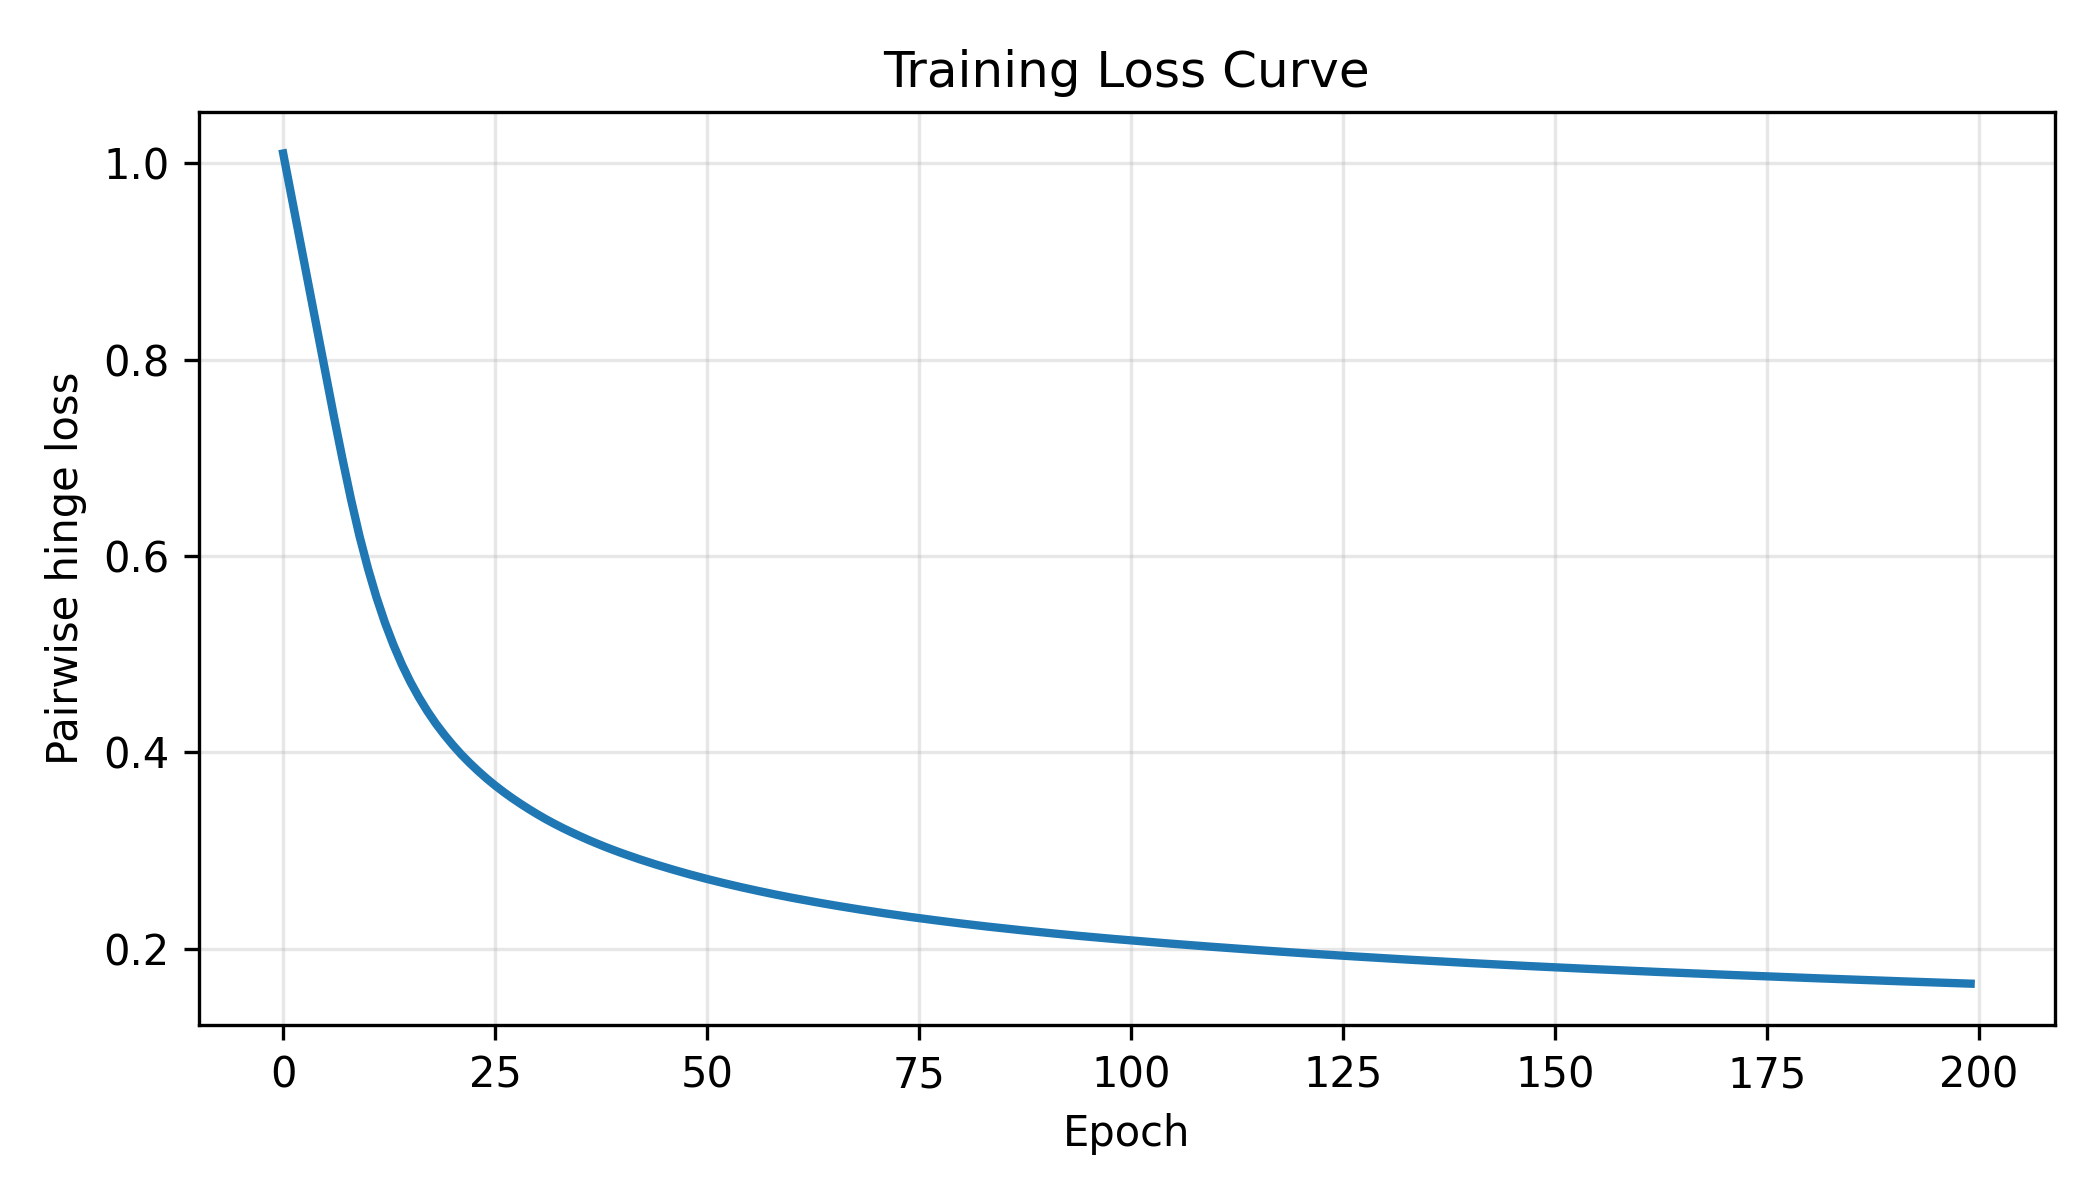
\includegraphics[width=0.85\textwidth]{figures/loss_curve.png}
    \caption{Đường cong pairwise hinge loss trong quá trình huấn luyện. Loss giảm nhanh ở các epoch đầu và tiếp tục giảm chậm dần về sau, cho thấy quá trình tối ưu đang hội tụ.}
    \label{fig:loss-curve}
\end{figure}

Loss giảm mạnh ở giai đoạn đầu và giảm chậm dần về sau. Điều này phù hợp với gradient descent: ban đầu mô hình còn sai nhiều nên gradient lớn; khi số cặp vi phạm margin giảm, tốc độ cải thiện cũng nhỏ hơn.

\subsection{So sánh ranking thật và ranking dự đoán}

Hình~\ref{fig:ranking-comparison} so sánh thứ tự ranking thật và thứ tự ranking dự đoán sau khi huấn luyện.

\begin{figure}[H]
    \centering
    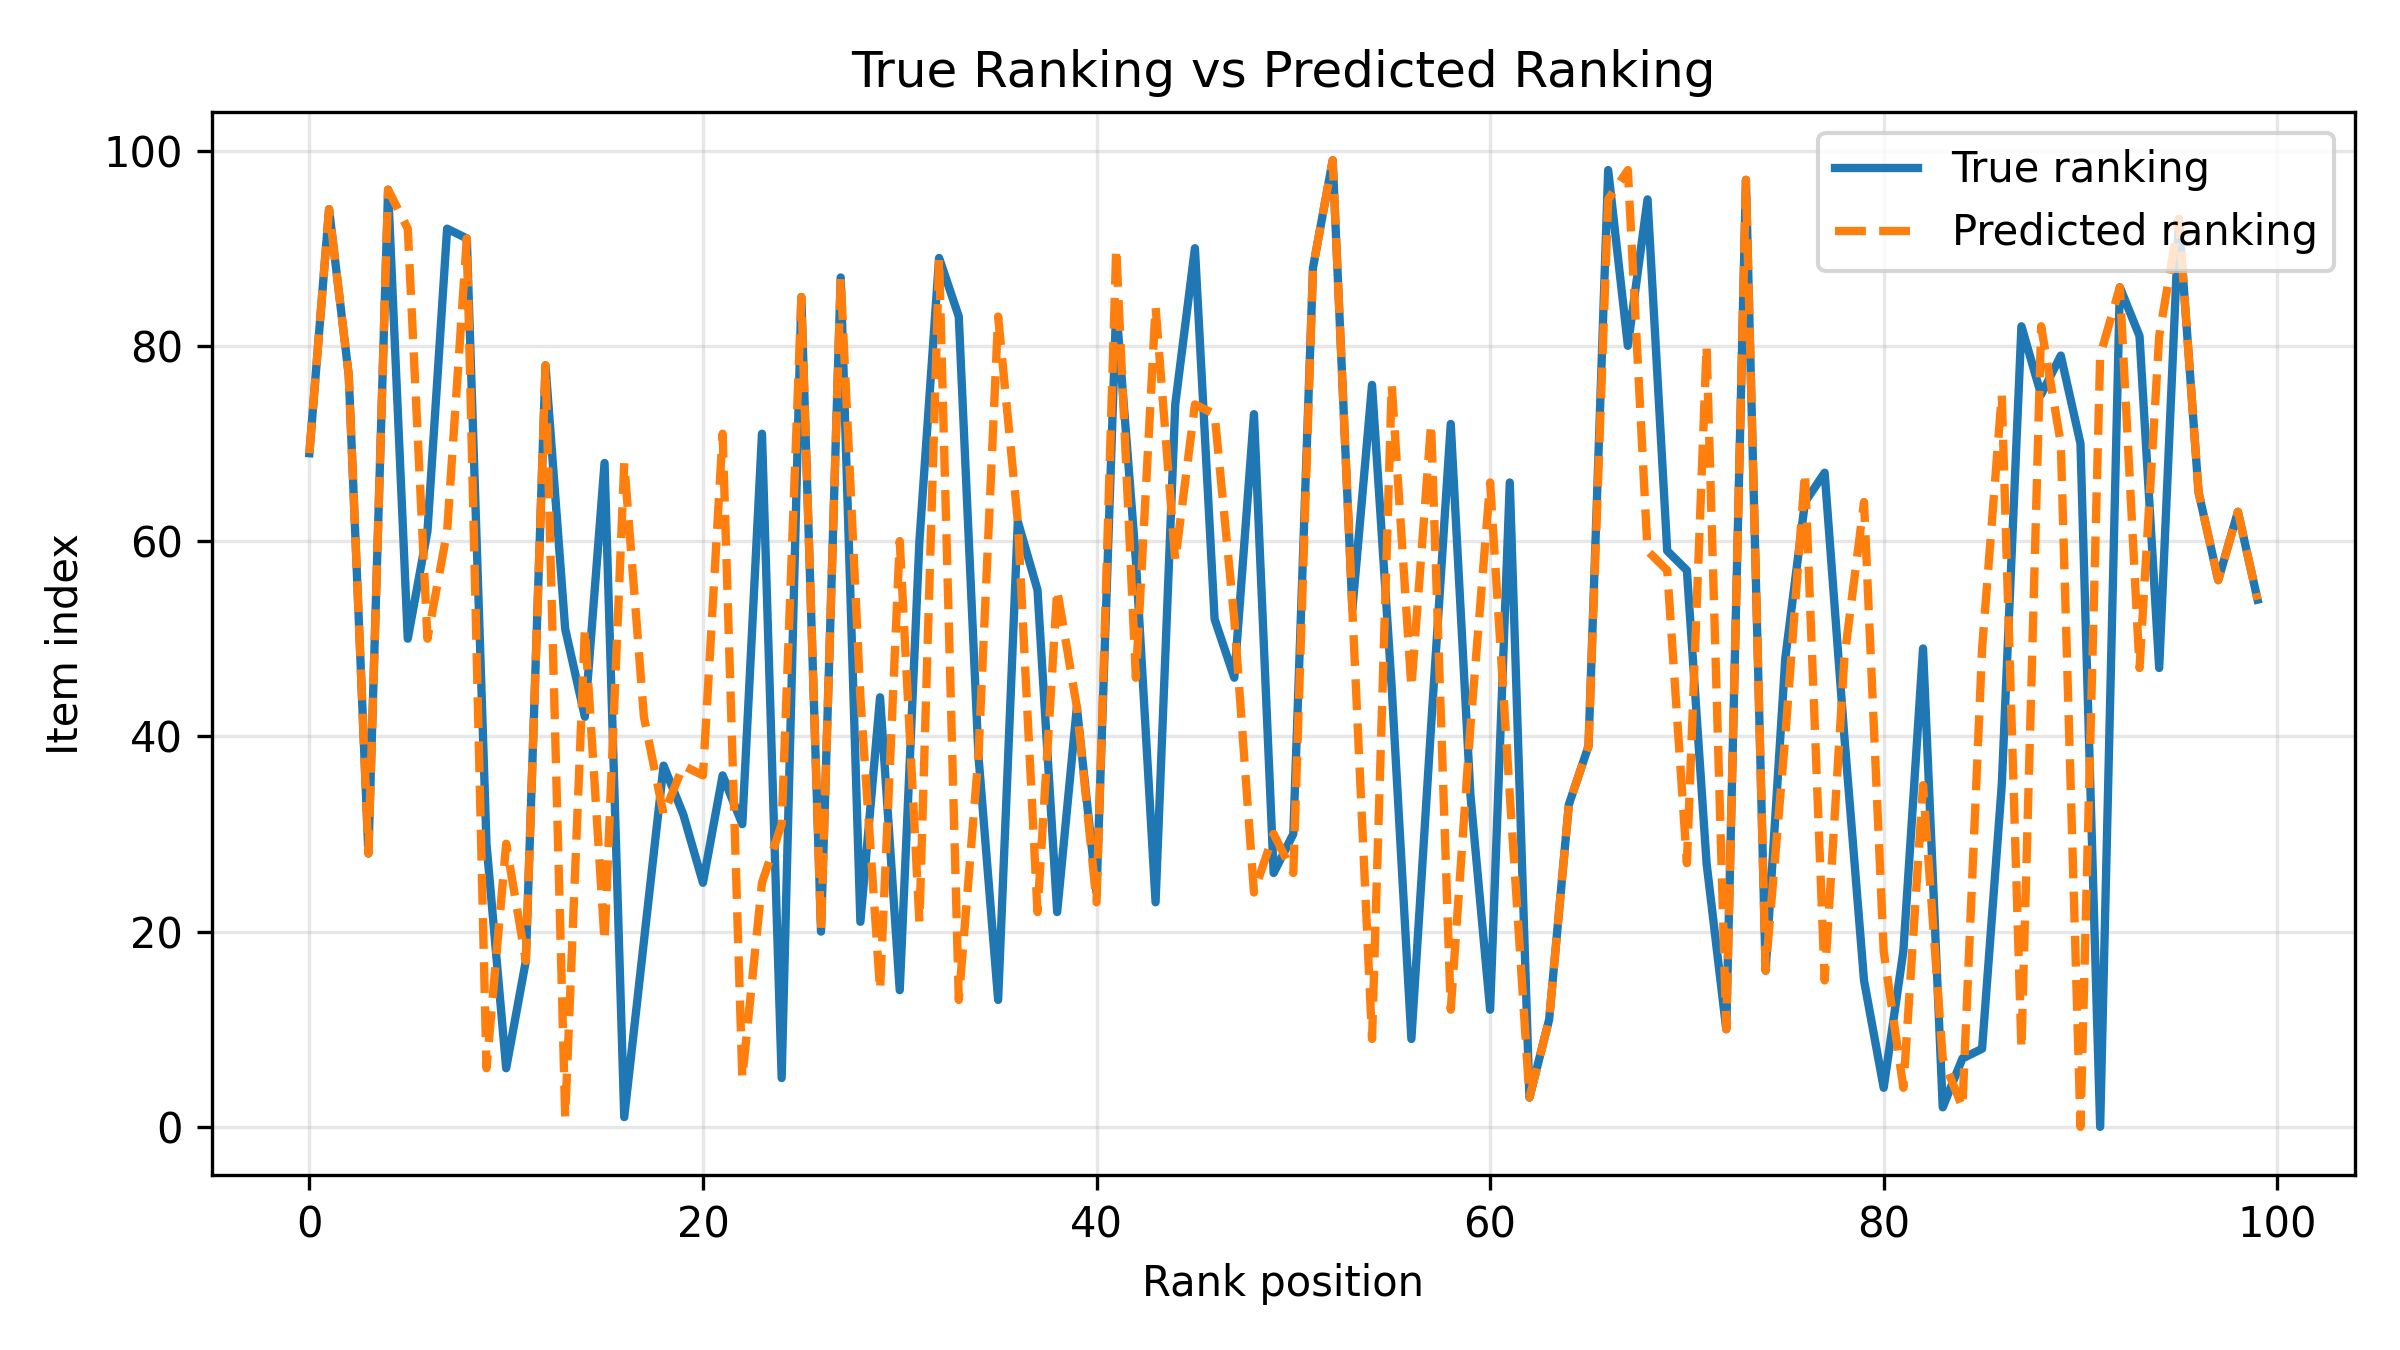
\includegraphics[width=0.9\textwidth]{figures/ranking_comparison.png}
    \caption{So sánh thứ tự ranking thật và ranking dự đoán. Hai đường càng gần nhau thì mô hình càng bảo toàn tốt quan hệ thứ tự giữa các mẫu.}
    \label{fig:ranking-comparison}
\end{figure}

Ranking dự đoán có xu hướng bám sát ranking thật. Tuy nhiên, do trục tung biểu diễn chỉ số mẫu theo từng vị trí xếp hạng, đồ thị có dạng dao động mạnh. Vì vậy, kết luận định lượng nên dựa chủ yếu vào pairwise accuracy, ranking loss và Kendall tau distance.

\subsection{Ảnh hưởng của nhiễu đến chất lượng ranking}

Để kiểm chứng ảnh hưởng của nhiễu, nhóm giữ cố định \(n=100\) và thay đổi độ lệch chuẩn nhiễu:
\[
    \sigma \in \{0.0,0.1,0.3,0.5,1.0\}.
\]

Kết quả được trình bày trong Bảng~\ref{tab:noise-results} và Hình~\ref{fig:noise-experiment}.

\begin{table}[H]
\centering
\caption{Ảnh hưởng của nhiễu đến chất lượng ranking}
\label{tab:noise-results}
\begin{tabular}{rrrrr}
\toprule
\textbf{Noise} & \textbf{Pairwise acc.} & \textbf{Ranking loss} & \textbf{Kendall tau} & \textbf{Top-10 overlap} \\
\midrule
0.0 & 0.996162 & 0.003838 & 0.003838 & 1.0 \\
0.1 & 0.985455 & 0.014545 & 0.014545 & 0.9 \\
0.3 & 0.945859 & 0.054141 & 0.054141 & 1.0 \\
0.5 & 0.914141 & 0.085859 & 0.085859 & 0.8 \\
1.0 & 0.838384 & 0.161616 & 0.161616 & 0.7 \\
\bottomrule
\end{tabular}
\end{table}

\begin{figure}[H]
    \centering
    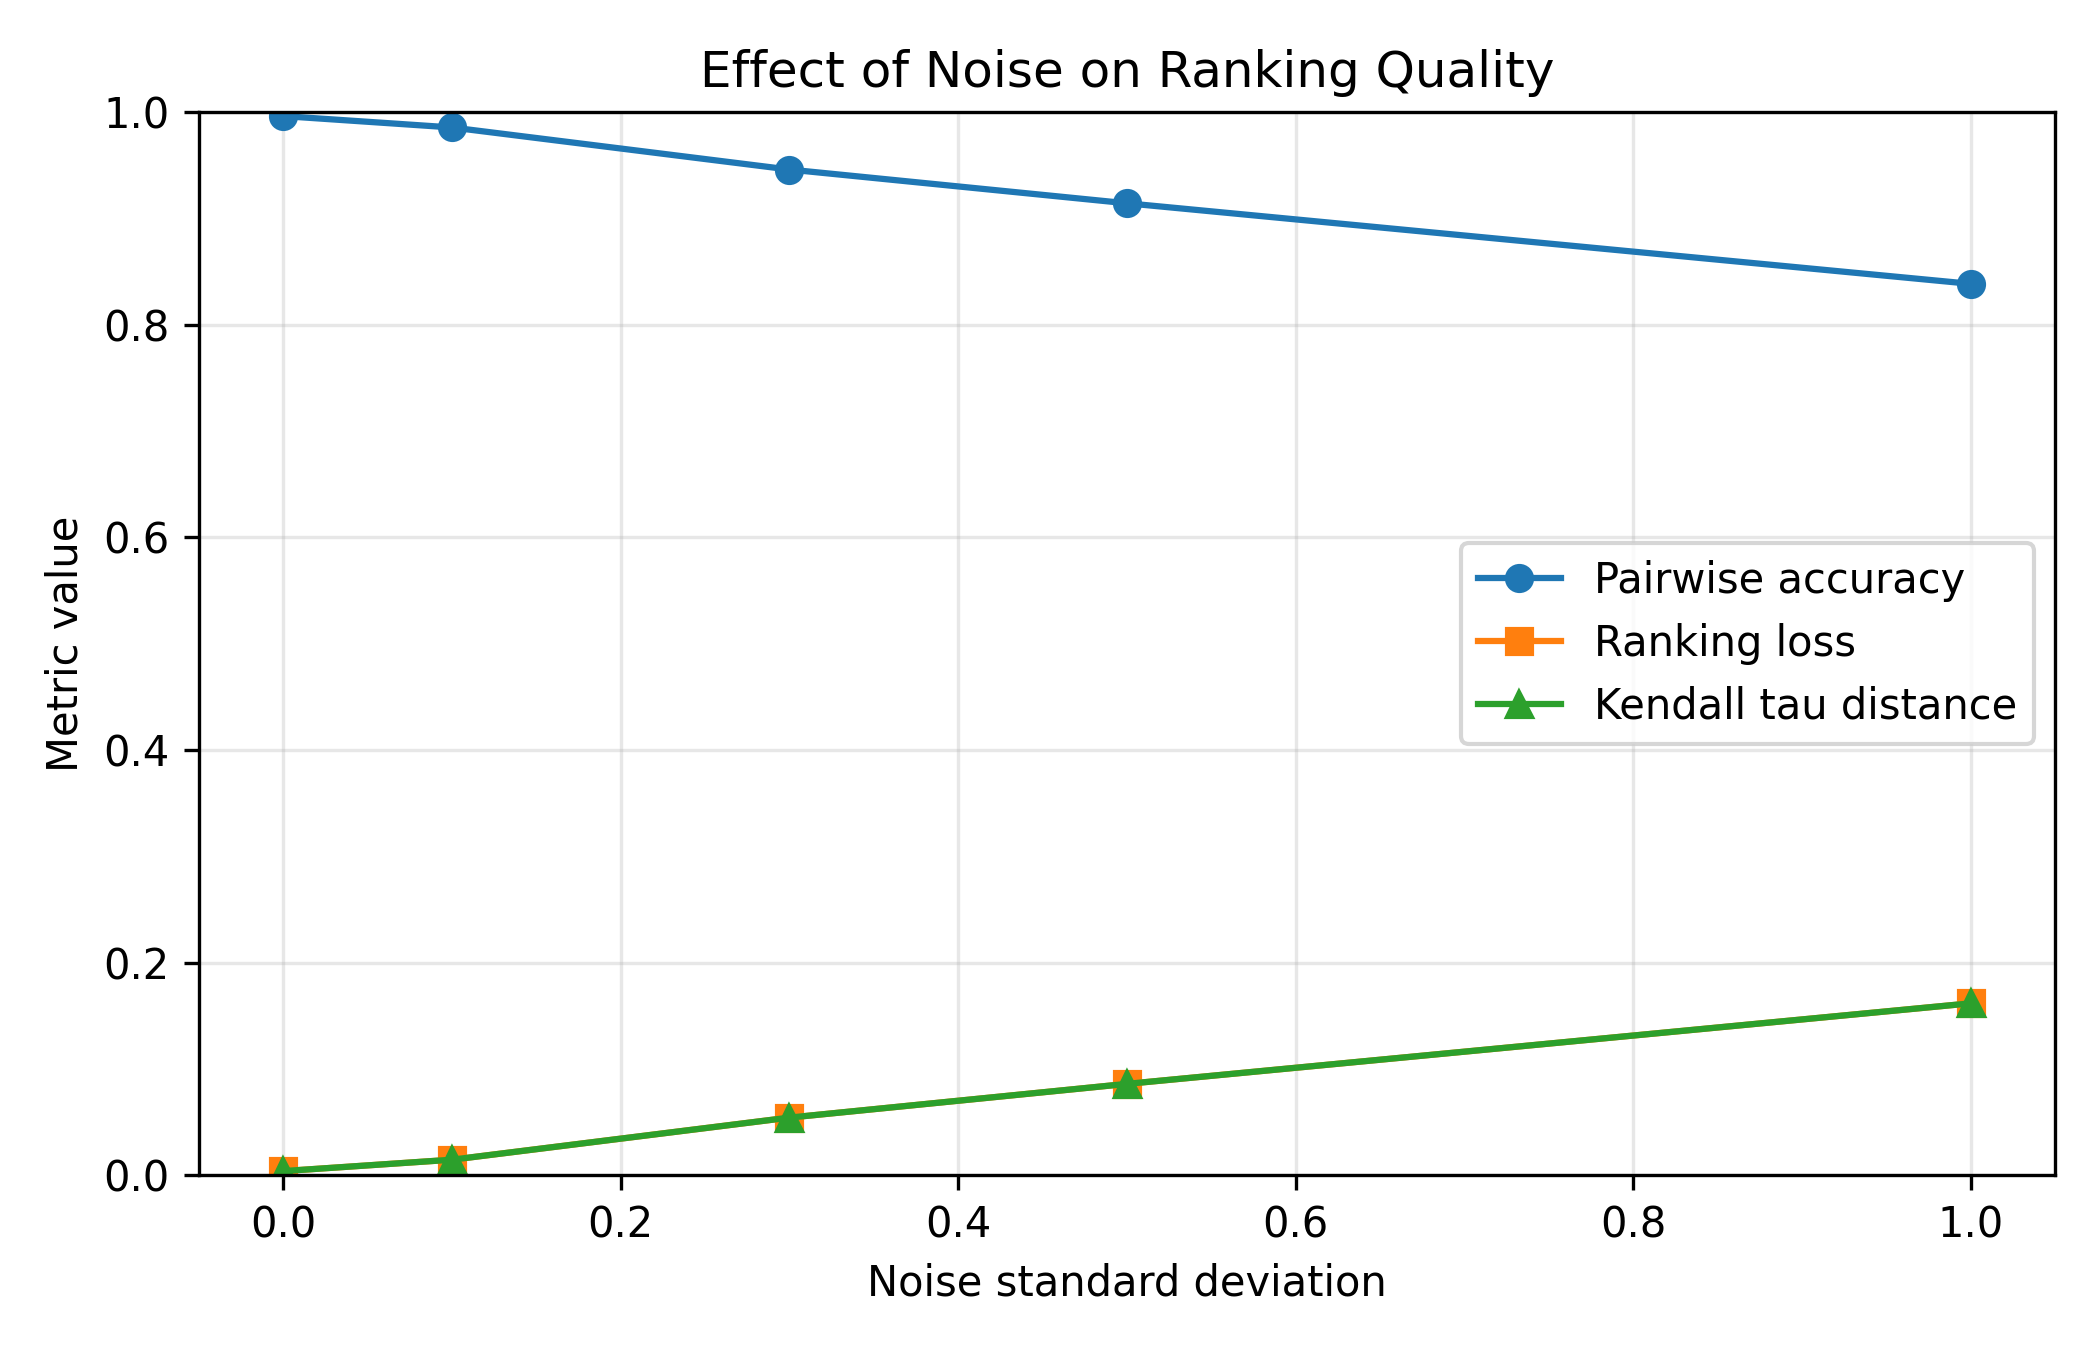
\includegraphics[width=0.9\textwidth]{figures/noise_experiment.png}
    \caption{Ảnh hưởng của độ lệch chuẩn nhiễu đến chất lượng ranking. Khi nhiễu tăng, pairwise accuracy giảm, trong khi ranking loss và Kendall tau distance tăng.}
    \label{fig:noise-experiment}
\end{figure}

Khi nhiễu tăng, chất lượng ranking giảm rõ rệt. Với \(\sigma=0.0\), dữ liệu gần như hoàn toàn tuyến tính nên pairwise accuracy đạt khoảng \(0.996\). Khi \(\sigma=1.0\), pairwise accuracy giảm xuống khoảng \(0.838\), ranking loss tăng lên khoảng \(0.162\), và top-10 overlap giảm còn \(0.7\). Điều này cho thấy nhiễu làm quan hệ ưu tiên kém ổn định hơn, khiến mô hình khó khôi phục ranking đúng.

\subsection{Ảnh hưởng của kích thước mẫu}

Trong thí nghiệm tiếp theo, nhóm cố định \(\sigma=0.1\) và thay đổi số lượng mẫu:
\[
    n \in \{20,50,100,200,500\}.
\]

Kết quả được trình bày trong Bảng~\ref{tab:sample-size-results} và Hình~\ref{fig:sample-size-experiment}.

\begin{table}[H]
\centering
\caption{Ảnh hưởng của kích thước mẫu đến chất lượng ranking}
\label{tab:sample-size-results}
\begin{tabular}{rrrrr}
\toprule
\textbf{Số mẫu} & \textbf{Pairwise acc.} & \textbf{Ranking loss} & \textbf{Kendall tau} & \textbf{Top-10 overlap} \\
\midrule
20  & 0.957895 & 0.042105 & 0.042105 & 0.9 \\
50  & 0.969796 & 0.030204 & 0.030204 & 0.9 \\
100 & 0.985455 & 0.014545 & 0.014545 & 0.9 \\
200 & 0.985829 & 0.014171 & 0.014171 & 0.9 \\
500 & 0.984858 & 0.015142 & 0.015142 & 1.0 \\
\bottomrule
\end{tabular}
\end{table}

\begin{figure}[H]
    \centering
    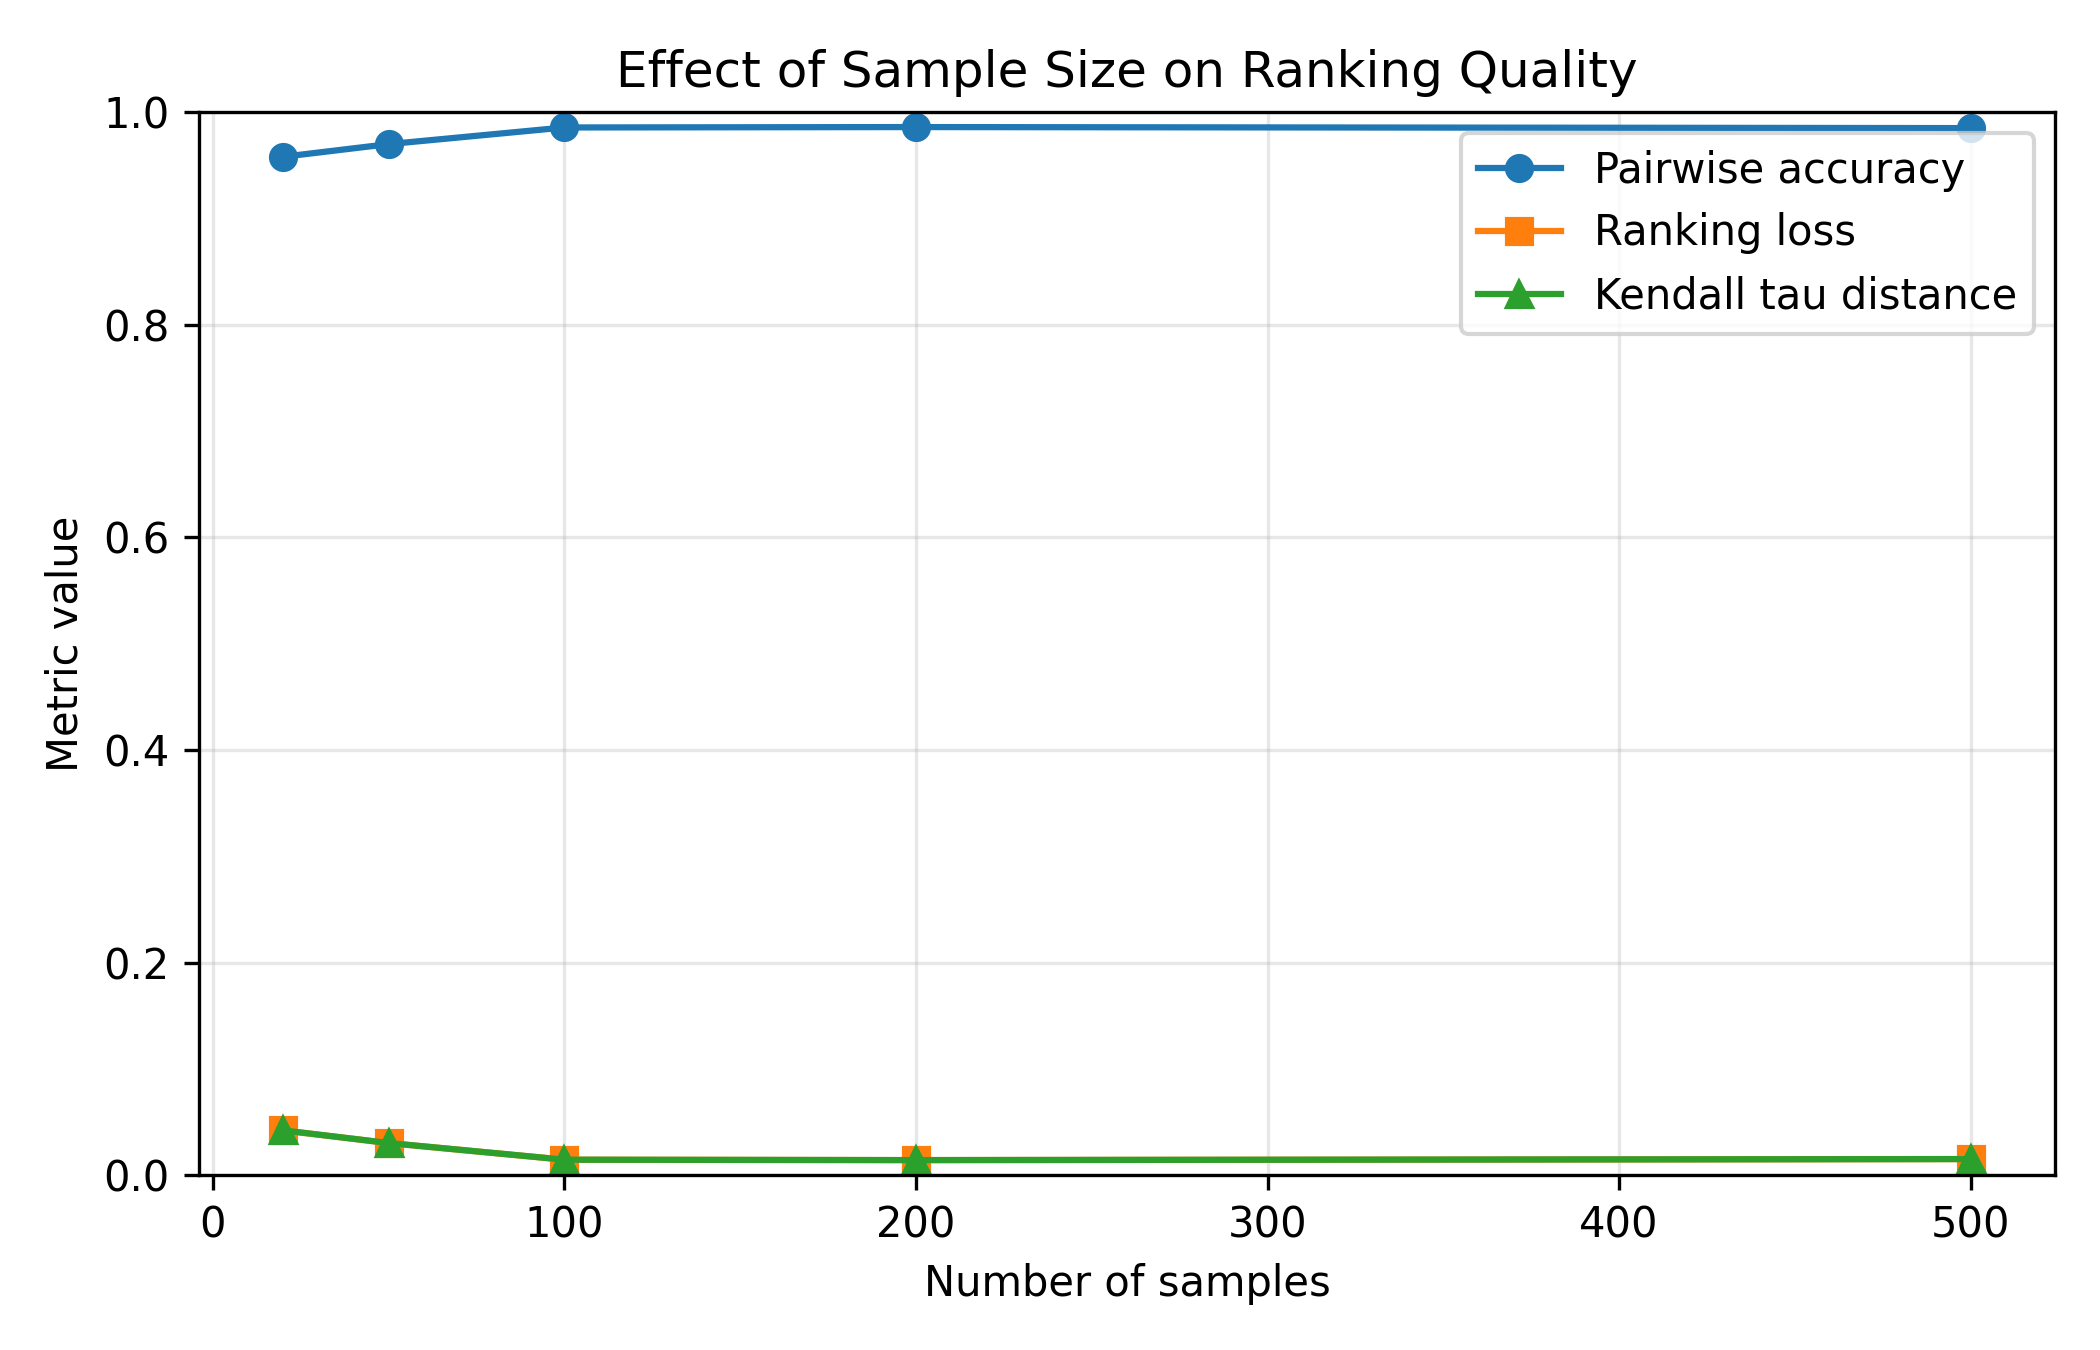
\includegraphics[width=0.9\textwidth]{figures/sample_size_experiment.png}
    \caption{Ảnh hưởng của kích thước mẫu đến chất lượng ranking. Khi số mẫu tăng, pairwise accuracy nhìn chung tăng và ranking loss giảm, sau đó ổn định ở mức tốt.}
    \label{fig:sample-size-experiment}
\end{figure}

Khi số mẫu tăng từ \(20\) lên \(100\), pairwise accuracy tăng và ranking loss giảm. Khi số mẫu tiếp tục tăng lên \(200\) và \(500\), chất lượng ranking duy trì ở mức cao. Do dữ liệu được sinh từ mô hình tuyến tính đơn giản và nhiễu nhỏ, mô hình đã đạt kết quả tốt ngay cả khi số mẫu chưa quá lớn.

\subsection{Khả năng tái tạo thực nghiệm}

Các thực nghiệm được thiết kế để có thể tái tạo. Nhóm sử dụng random seed cố định trong quá trình sinh dữ liệu, khởi tạo mô hình và chạy thực nghiệm. Các tham số như số mẫu, số đặc trưng, số epoch, learning rate và regularization đều được ghi rõ.

Các kết quả được lưu thành các file CSV:
\begin{itemize}
    \item \texttt{results/tables/main\_results.csv}: kết quả thực nghiệm chính.
    \item \texttt{results/tables/noise\_results.csv}: kết quả thí nghiệm thay đổi mức nhiễu.
    \item \texttt{results/tables/sample\_size\_results.csv}: kết quả thí nghiệm thay đổi kích thước mẫu.
\end{itemize}

Các hình minh hoạ được lưu trong thư mục \texttt{figures/}. Các thư viện chính gồm \texttt{numpy}, \texttt{matplotlib}, \texttt{csv} và \texttt{pathlib}. Phiên bản cụ thể của các thư viện được liệt kê trong file \texttt{requirements.txt}.

\subsection{Nhận xét chung}

Các thực nghiệm cho thấy mô hình pairwise ranking tuyến tính có thể học tốt quan hệ ưu tiên khi dữ liệu được sinh từ một hàm tuyến tính. Điều này thể hiện qua pairwise accuracy cao, ranking loss thấp và top-10 overlap tốt.

Đường cong loss cho thấy quá trình huấn luyện có xu hướng hội tụ. Khi nhiễu tăng, số lượng cặp bị đảo thứ tự tăng lên, làm giảm pairwise accuracy và tăng ranking loss. Khi kích thước mẫu tăng, mô hình quan sát được nhiều cặp ưu tiên hơn nên học ổn định hơn, dù mức cải thiện sau \(100\) mẫu không còn quá lớn.

Nhìn chung, kết quả thực nghiệm phù hợp với lý thuyết về pairwise learning-to-rank: mô hình học một hàm scoring sao cho bảo toàn nhiều nhất có thể các quan hệ ưu tiên giữa các cặp mẫu.
